\setlength{\columnsep}{3pt}
\begin{flushleft}
	\bigskip
	\paragraph{What is vi editor?}
	\begin{itemize}
		\item Vi is a free and open source, screen-based text editor program for Linux/Unix OS.
	\end{itemize}


	\paragraph{What is vim editor?}
	\begin{itemize}
		\item Vim is an advance version of vi.
		
	We are going to explore "vim" editor in detail as it is more advance than "vi".

	\paragraph{How to use vi or vim editor?}
			\bigskip
			\begin{tcolorbox}[breakable,notitle,boxrule=1pt,colback=black,colframe=black]
				\color{green}
				\fontdimen2\font=1em
				\$ vim one.txt
				\newline
				or
				\newline
				\$ vi one.txt
				\fontdimen2\font=4pt
			\end{tcolorbox}
			This will open an editor in front of you as shown:
			\begin{figure}[h!]
			\centering
			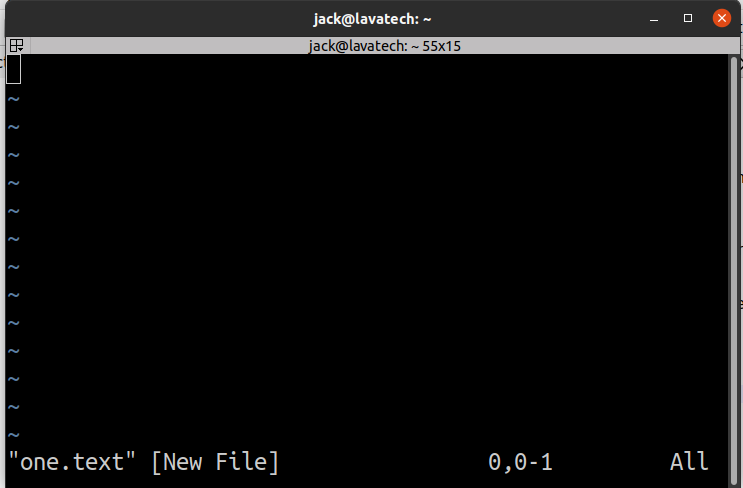
\includegraphics[scale=.4]{content/chapter3/images/vim.png}
			\caption{Vim Editor}
			\label{fig:vim_editor}
		\end{figure}
	
	\end{itemize}
	
\end{flushleft}

\newpage





